\section{EiffelStudio}
\label{implementation_eiffelstudio}
In continuation of the \textsc{ui} discussion in the previous section, this section will examine how the actual code behind this \textsc{ui} works. Also it will be analyzed, how EiffelStudio acts to switch to the appropriate view, and how text inside the textual views are generated. All classes in figure \ref{fig:extractor_structure} will be described on a conceptual level to give the reader an idea how views are handled. To get a deeper understanding it is suggested to study the source code itself.

\begin{figure}[H]
\centering

\includegraphics[scale=0.8]{images/es0.png}
\caption{View bar in EiffelStudio}
\label{fig:EiffelStudio0}
\end{figure}

In figure \ref{fig:EiffelStudio0} the toolbar for changing between the standard views of EiffelStudio is shown, from left to right, \textit{Basic text view}, \textit{Clickable view}, \textit{Flat view}, \textit{Contract view}, and \textit{Interface view}. Each of these views are represented by a subclass of \textsc{eb$\_$class$\_$text$\_$for- matter}, and as such, to keep in line with EiffelStudio's structure, any new views also should be as such. A formatter is responsible for displaying text in a text area. This concept is illustrated by figure \ref{fig:extractor_structure}, where it can be seen that a subclass of the class text formatter has been made for formal textual \bon. Accordingly, a similar class has been implemented for informal \bon{}. The changing between these views is handled by a development window, the purpose of which is to be a container for project tools, in this case a textual view. The \textsc{textual$\_$bon$\_$format$\_$tables} class is a shared format table that contains metadata about the view selected by the user. The \textsc{text$\_$formatter$\_$decorator} is responsible for decorating text to be shown, and works as a mediator between the output strategy (explained next) and the formatter. This text formatter decorator also works as the link from the internal representation back to EiffelStudio (described by figure \ref{fig:bon_extraction_4}), as it processes text given from the internal \bon{} representation as tokens. The output strategy's (in figure \ref{fig:extractor_structure}: \textsc{textual$\_$bon$\_$formal$\_$output$\_$strategy}) function is to generate some sort of textual output based on an abstract syntax. In the case of the views already in place in EiffelStudio, the output strategy works as a visitor that traverses through the abstract Eiffel syntax and generates decorated text that way. As it was decided not to use a visitor pattern for the textual \bon{} extractor, the output strategy's role is to initialize the meta-object (mentioned in section \ref{design-bon-extraction}) and then start the generation of the textual \bon.

\begin{figure}[H]
\centerline{
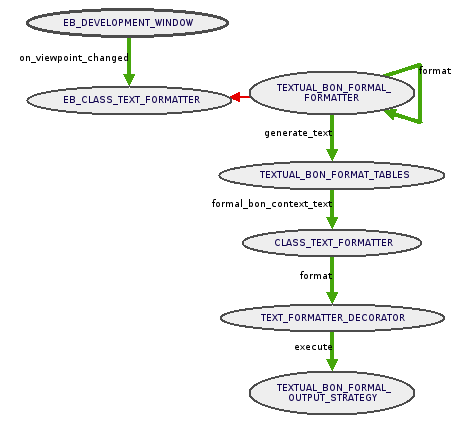
\includegraphics[scale=0.7]{images/BON-extractor-structure-large.png}
}
\caption{Structure of the \bon{} extractor's interaction with EiffelStudio for formal \bon.}
\label{fig:extractor_structure}
\end{figure}

\subsection{BON Syntax Highlighting}
At the heart of the syntax highlighter for textual \bon{} in EiffelStudio is the scanner class \textsc{editor\_textual\_bon\_scanner}. Like the textual \bon{} scanner used for type checking, this scanner class is also generated by the \textit{gelex} tool. The syntax highlighting scanner for textual \bon{} is a modified version of an already existing scanner for syntax highlighting made for the Eiffel views in EiffelStudio. 

Whenever an element that needs highlighting is encountered, such as a keyword or a symbol, an appropriate subtype of the class \textsc{editor\_token} is instantiated by the scanner. These are the same token classes that EiffelStudio makes use of when highlighting Eiffel syntax. The highlighted text in a view is thus represented as a stream of tokens, each of them appropriately decorated with a color chosen through the preferences of EiffelStudio. For a uniform experience of switching between an Eiffel view and a textual \bon{} view, the colors for each of the different syntactic elements are the same for \bon{} as they are for Eiffel.

The extracted \bon{} does not rely on this highlighting scanner, however. Instead, whenever a user switches to a textual \bon{} view, the extractor code generates the aforementioned stream of decorated tokens while traversing the internal \bon{} representation, after which these tokens are handed back to EiffelStudio to be displayed. As such, highlighting and extraction is done simultaneously.

The highlighting scanner's raison d'\^etre is thus future use when actually editing the extracted \bon{}. At this point, the scanner has not been integrated into EiffelStudio, but this integration should be possible through the class \textsc{eb\_editor} or has subclass thereof.
